% -----------------------------------------------
% Template for SMAC SMC 2013
% adapted and corrected from the template for SMC 2012, which was adapted from that of SMC 2011
% further updated for TENOR 2015 and 2016
% -----------------------------------------------

\documentclass{article}
\usepackage{tenor2016}
%\usepackage{times}
\usepackage{ifpdf}
\usepackage[english]{babel}
%\usepackage{cite}

%%%%%%%%%%%%%%%%%%%%%%%% Some useful packages %%%%%%%%%%%%%%%%%%%%%%%%%%%%%%%
%%%%%%%%%%%%%%%%%%%%%%%% See related documentation %%%%%%%%%%%%%%%%%%%%%%%%%%
%\usepackage{amsmath} % popular packages from Am. Math. Soc. Please use the 
%\usepackage{amssymb} % related math environments (split, subequation, cases,
%\usepackage{amsfonts}% multline, etc.)
%\usepackage{bm}      % Bold Math package, defines the command \bf{}
%\usepackage{paralist}% extended list environments
%%subfig.sty is the modern replacement for subfigure.sty. However, subfig.sty 
%%requires and automatically loads caption.sty which overrides class handling 
%%of captions. To prevent this problem, preload caption.sty with caption=false 
%\usepackage[caption=false]{caption}
%\usepackage[font=footnotesize]{subfig}


%user defined variables
\def\papertitle{INScore expressions to compose symbolic scores}
\def\authors{G. Lepetit-Aimon \qquad D. Fober \qquad Y. Orlarey \qquad S. Letz}
\def\firstauthor{Gabriel Lepetit-Aimon}
\def\secondauthor{Dominique Fober}
\def\thirdauthor{Yann Orlarey}
\def\fourthauthor{Stéphane Letz}

% adds the automatic
% Saves a lot of ouptut space in PDF... after conversion with the distiller
% Delete if you cannot get PS fonts working on your system.

% pdf-tex settings: detect automatically if run by latex or pdflatex
\newif\ifpdf
\ifx\pdfoutput\relax
\else
   \ifcase\pdfoutput
      \pdffalse
   \else
      \pdftrue
\fi

\ifpdf % compiling with pdflatex
  \usepackage[pdftex,
    pdftitle={\papertitle},
    pdfauthor={\firstauthor, \secondauthor, \thirdauthor},
    bookmarksnumbered, % use section numbers with bookmarks
    pdfstartview=XYZ % start with zoom=100% instead of full screen; 
                     % especially useful if working with a big screen :-)
   ]{hyperref}
  %\pdfcompresslevel=9

  \usepackage[pdftex]{graphicx}
  % declare the path(s) where your graphic files are and their extensions so 
  %you won't have to specify these with every instance of \includegraphics
  \graphicspath{{./figures/}}
  \DeclareGraphicsExtensions{.pdf,.jpeg,.png}

  \usepackage[figure,table]{hypcap}

\else % compiling with latex
  \usepackage[dvips,
    bookmarksnumbered, % use section numbers with bookmarks
    pdfstartview=XYZ % start with zoom=100% instead of full screen
  ]{hyperref}  % hyperrefs are active in the pdf file after conversion

  \usepackage[dvips]{epsfig,graphicx}
  % declare the path(s) where your graphic files are and their extensions so 
  %you won't have to specify these with every instance of \includegraphics
  \graphicspath{{./figures/}}
  \DeclareGraphicsExtensions{.eps}

  \usepackage[figure,table]{hypcap}
\fi

%setup the hyperref package - make the links black without a surrounding frame
\hypersetup{
    colorlinks,%
    citecolor=black,%
    filecolor=black,%
    linkcolor=black,%
    urlcolor=black
}


% Title.
% ------
\title{\papertitle}

% Authors
% Please note that submissions are NOT anonymous, therefore 
% authors' names have to be VISIBLE in your manuscript. 
%
% Single address
% To use with only one author or several with the same address
% ---------------
\oneauthor
   {\authors} {Grame \\ %
  Centre nationale de création musicale \\
  Lyon - France \\
     {\tt \href{mailto:gabriel.lepetit.aimon@grame.fr}{gabriel.lepetit.aimon@grame.fr}}}

%Two addresses
%--------------
% \twoauthors
%   {\firstauthor} {Grame \\ %
%     {\tt \href{mailto:gabriel.lepetit.aimon@grame.fr}{gabriel.lepetit.aimon@grame.fr}}}
%   {\secondauthor} {Grame \\ %
%     {\tt \href{mailto:fober@grame.fr}{fober@grame.fr}}}

% Three addresses
% --------------
% \threeauthors
%   {\firstauthor} {Affiliation1 \\ %
%     {\tt \href{mailto:author1@adomain.org}{author1@adomain.org}}}
%   {\secondauthor} {Affiliation2 \\ %
%     {\tt \href{mailto:author2@adomain.org}{author2@adomain.org}}}
%   {\thirdauthor} { Affiliation3 \\ %
%     {\tt \href{mailto:author3@adomain.org}{author3@adomain.org}}}


% ***************************************** the document starts here ***************
\begin{document}
%
\capstartfalse
\maketitle
\capstarttrue
%
\begin{abstract}
INScore is an environment for the design of augmented interactive music scores turned to non-conventional use of music notation. The environment allows arbitrary graphic resources to be used and composed for the music representation. It supports symbolic music notation, described using Guido Music Notation or MusicXML formats. The environment has been extended to provided score level composition using a set of operators that consistently take scores as arguments to compute new scores as output. INScore API supports now \emph{scores expressions} both at OSC and at scripting levels. The work is based on a previous research that solved the issues of the notation consistency accross scores composition. This paper focuses on the language level and explains the different strategies to evaluate score expressions.
\end{abstract}
%

\section{Introduction}\label{sec:introduction}

Contemporary music creation poses numerous challenges to the music notation. Spatialized music, new instruments, gesture based interactions, real-time and interactive scores, are among the new domains that are now commonly explored by artists. 
Classical music notation doesn't cover the needs of these new musical forms and numerous research and approaches have recently emerged, testifying to the maturity of the music notation domain, in the light of computer tools for music notation and representation.
Issues like writing spatialized music \cite{Ellberger_tenor2015}, addressing new instruments \cite{tmays:2014} or new interfaces \cite{kschlei:2015} (to cite just a few), are now subject of active research and proposals.

Interactive music and real-time scores are also representative of an expanding domain in the music creation field. The advent of the digital score and the maturation of the computer tools for music notation and representation constitute the basement for the development of this musical form, which is often grounded on non-traditional music representation \cite{RSmith_tenor2015} \cite{Hope_tenor2015} but may also use the common music notation \cite{Hoadley12,hoadley14}. 

In order to address the notations challenges mentionned above, INScore \cite{Fober:12a,fober14c} has been designed as an environment opened to non-conventional music representation (although it supports symbolic notation), and turned to real-time and interactive use \cite{Fober:13b, Fober:14b}. It is clearly focused on music representation only and in this way, differs from tools integrated into programming environments like Bach \cite{agostini12b} or MaxScore \cite{didko08}. 

INScore has been extended with \emph{score expressions} that provide symbolic scores composition features (e.g., putting scores in sequence or in parallel). Building new scores from existing scores at symbolic  level is not new. Haskell is providing such features with the \texttt{music-xxx} package... (???). Freeman and Lee proposed score composition operations in a real-time and interactive notation context \cite{Lee:2013}. Regarding the score operations used by INScore, they are imported from a previous work \cite{fober12b} that was focusing on the music notation consistency through arbitrary composition. 

The novelty of the proposed approach relies on the dynamic aspects of the scores composition operations, as well as on the persistence of the score expressions. A score may be composed as an arbitrary graph of score expressions and equipped with a fine control over the changes propagation.

The paper introduces first the score composition expressions. Next, the different evaluations strategies are explained and illustrated with examples. The articulation with the INScore environment is presented in detail and followed by concrete use cases. A generalization of this approach is finally proposed in the concluding section.  




\section{Typeset Text}\label{sec:typeset_text}



\section{Headings}
First level headings are in Times 12pt bold,
centered with 1 line of space above the section head, and 1/2 space below it.
For a section header immediately followed by a subsection header, the space 
should be merged.

\subsection{Second Level Headings}
Second level headings are in Times 10pt bold, flush left,
with 1 line of space above the section head, and 1/2 space below it.
The first letter of each significant word is capitalized.


\section{Floats and equations}

\subsection{Equations}
Equations of importance, 
or to which you refer later,
should be placed on separated lines and numbered.
The number should be on the right side, in parentheses.
\begin{equation}
E=mc^{2+\delta}.
\label{eq:Emc2}
\end{equation}
Refer to equations like so:
As (\ref{eq:Emc2}) shows, 
I do not completely trust Special Relativity.

\subsection{Figures, Tables and Captions}
\begin{table}[h]
 \begin{center}
 \begin{tabular}{|l|l|}
  \hline
  String value & Numeric value \\
  \hline
  Hello TENOR  & 2016 \\
  \hline
 \end{tabular}
\end{center}
 \caption{Table captions should be placed below the table, exactly like this,
 but using words different from these.}
 \label{tab:example}
\end{table}

All artwork must be centered, neat, clean, and legible.
And if you include figures in your paper, instead of artwork,
please make sure they are centered, neat, clean,
and completely legible without super resolution imaging.
All lines should be thick and dark enough to be reproducible
even by a facsimile machine;
and figures should not be hand-drawn unless your hand is robotically precise.
Since the proceedings are distributed in electronic form only, 
we allow color to be used in figures;
but please check that your figures are 
coherent if they are printed in black-and-white.
For instance, to make your figures zing in several conditions,
vary line thickness, style, and color at the same time.

Numbers and captions of figures and tables always appear below the figure/table.
Leave 1 line space between the figure or table and the caption.
Figure and tables are numbered consecutively. 
Captions should be Times 10pt.
And try to make your captions sufficiently explain your figures and tables.
Place tables/figures in text as close to the reference as possible, 
and preferably at the top of the page.

Always refer to tables and figures in the main text, for example:
see Fig. \ref{fig:example} and \tabref{tab:example}.
Figures and tables may extend across both columns to a maximum width of 17.2cm.

Vectorial figures are preferred, e.g., eps.
When using \texttt{Matlab}, 
export using either (encapsulated) Postscript or PDF format. 
In order to optimize readability, 
the font size of text within a figure should be no smaller than
that of footnotes (8pt font-size). 
If you use bitmap figures, make sure that 
the resolution is high enough for print quality. 

%\begin{figure}[t]
%\centering
%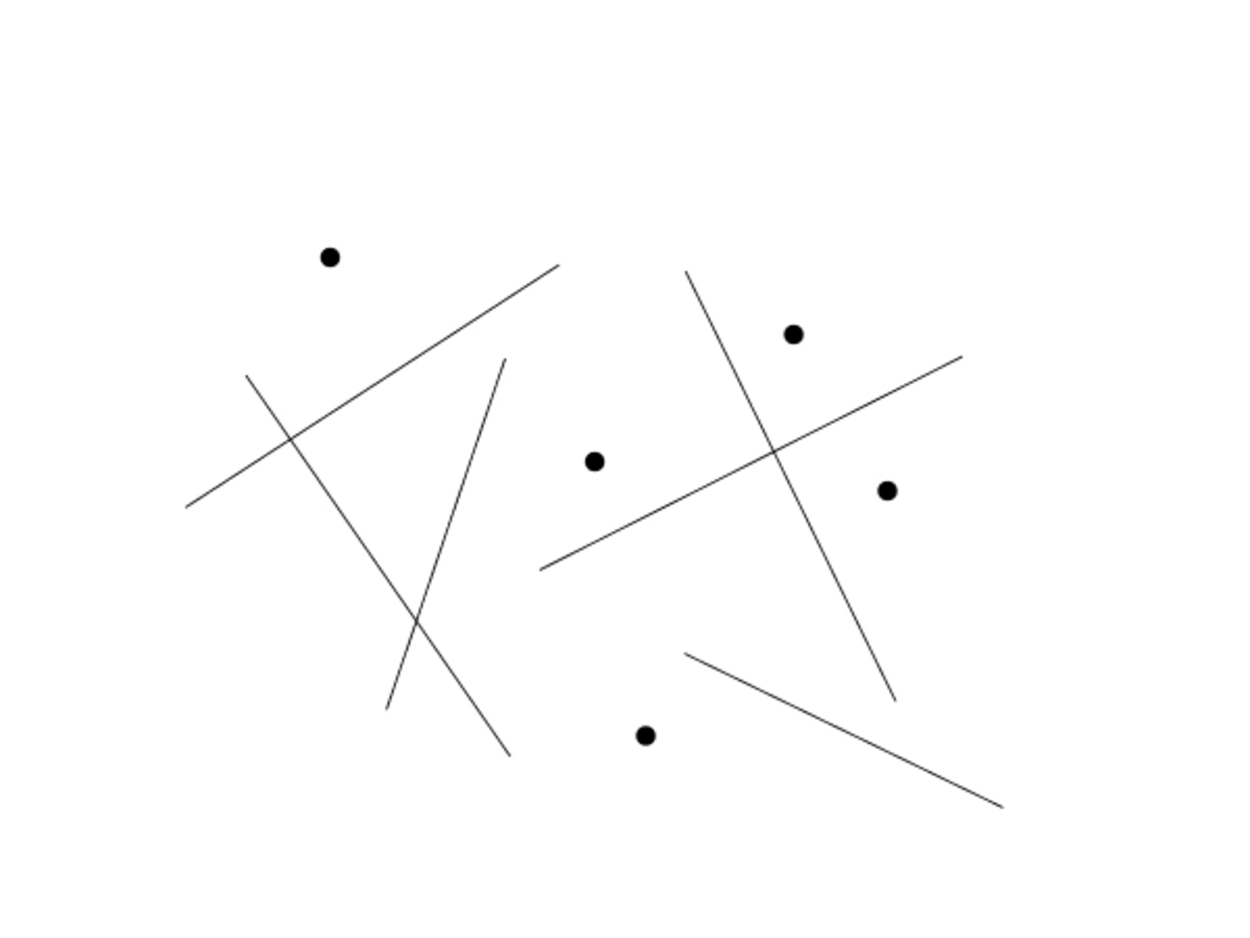
\includegraphics[width=0.9\columnwidth]{figure}
%\caption{Figure captions should be placed below the figure, 
%exactly like this.
%\label{fig:example}}
%\end{figure}

%\begin{figure}[t]
%\figbox{
%\subfloat[][]{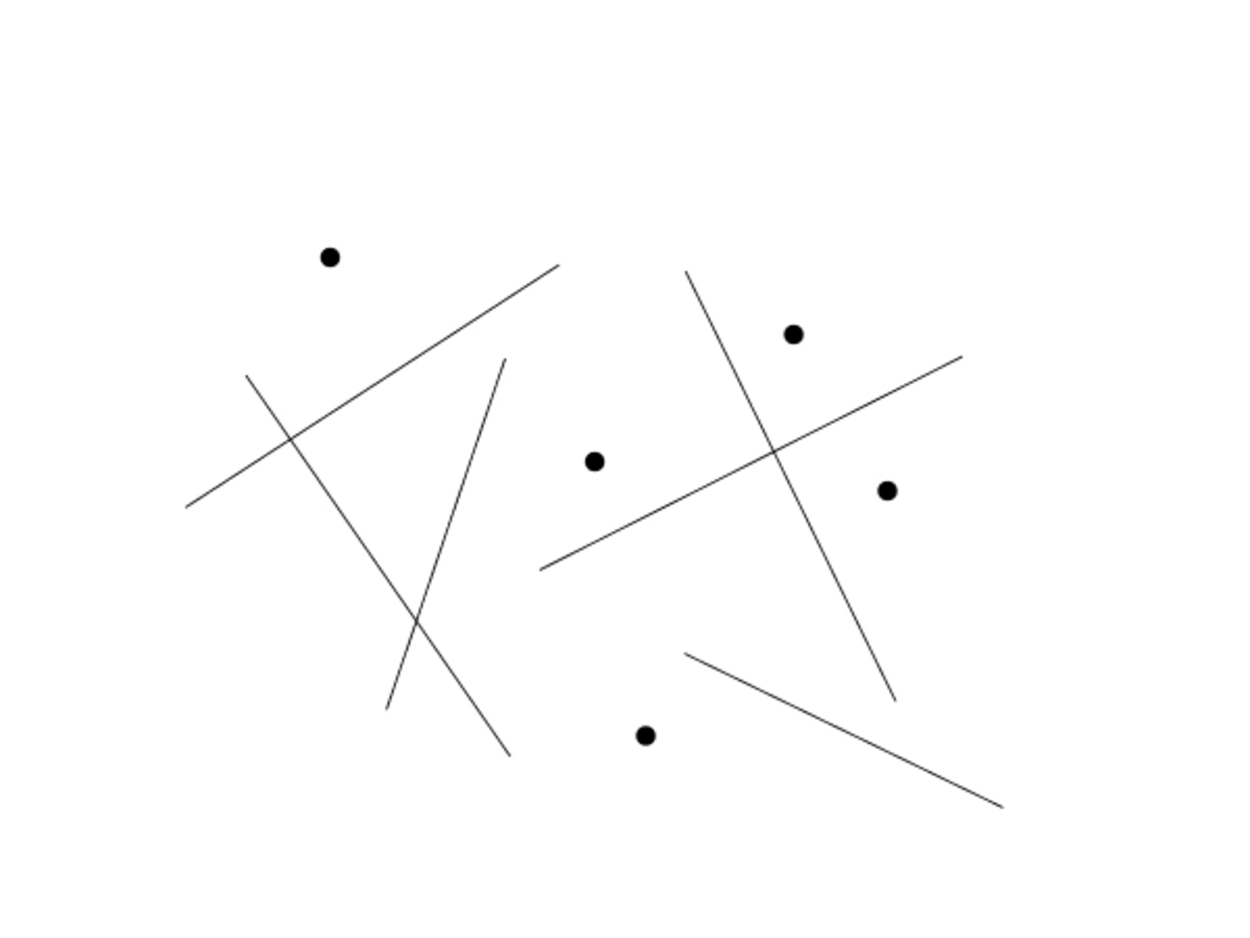
\includegraphics[width=60mm]{figure}\label{fig:subfigex_a}}\\
%\subfloat[][]{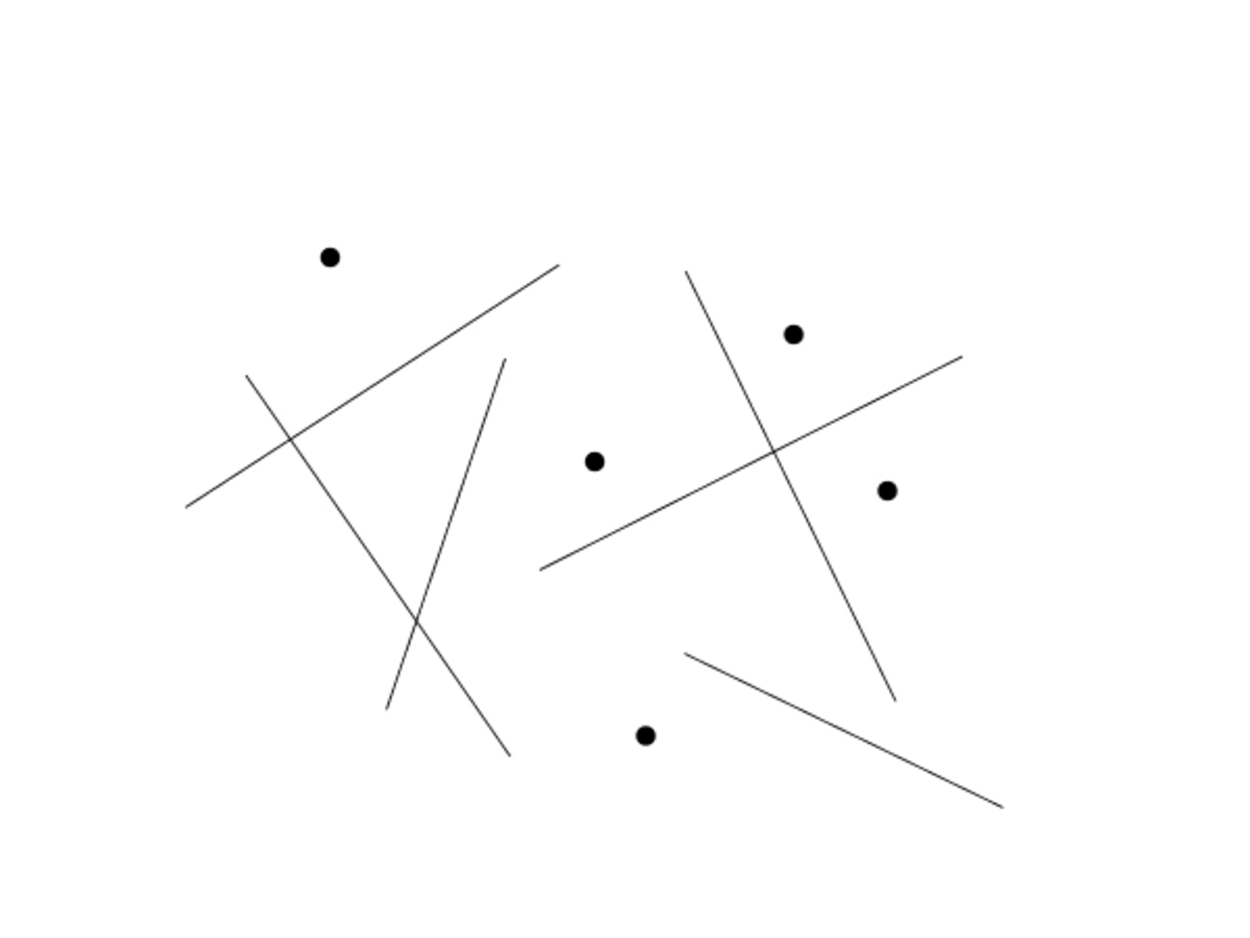
\includegraphics[width=80mm]{figure}\label{fig:subfigex_b}}
%}
%\caption{Here's an example using the subfig package.\label{fig:subfigex} }
%\end{figure}


\section{Conclusions}
To finish your full-length paper, end it with a conclusion;
and after careful editing and a final spell-cheek,
submit it through the \href{https://easychair.org/conferences/?conf=tenor2016}{\textcolor {magenta} {\underline {EasyChair Submission System}}}. 
\underline{Do not} send papers directly by e-mail.
%
\begin{acknowledgments}
You may acknowledge people, projects, 
funding agencies, etc. 
which can be included after the second-level heading
``Acknowledgments'' (with no numbering).
\end{acknowledgments} 

%%%%%%%%%%%%%%%%%%%%%%%%%%%%%%%%%%%%%%%%%%%%%%%%%%%%%%%%%%%%%%%%%%%%%%%%%%%%%
%bibliography here
\bibliography{../interlude}

\end{document}
